\pdfminorversion=4
\documentclass[aspectratio=169]{beamer}

\mode<presentation>
{
  \usetheme{default}
  \usecolortheme{default}
  \usefonttheme{default}
  \setbeamertemplate{navigation symbols}{}
  \setbeamertemplate{caption}[numbered]
  \setbeamertemplate{footline}[frame number]  % or "page number"
  \setbeamercolor{frametitle}{fg=white}
  \setbeamercolor{footline}{fg=black}
}

\usepackage[english]{babel}
\usepackage[utf8x]{inputenc}
\usepackage{tikz}
\usepackage{courier}
\usepackage{array}
\usepackage{bold-extra}
\usepackage{minted}
\usepackage[thicklines]{cancel}
\usepackage{fancyvrb}

\xdefinecolor{dianablue}{rgb}{0.18,0.24,0.31}
\xdefinecolor{darkblue}{rgb}{0.1,0.1,0.7}
\xdefinecolor{darkgreen}{rgb}{0,0.5,0}
\xdefinecolor{darkgrey}{rgb}{0.35,0.35,0.35}
\xdefinecolor{darkorange}{rgb}{0.8,0.5,0}
\xdefinecolor{darkred}{rgb}{0.7,0,0}
\xdefinecolor{mauve}{rgb}{0.58,0,0.82}
\xdefinecolor{brown}{rgb}{0.5,0.16,0.16}
\xdefinecolor{reallydarkgreen}{rgb}{0,0.25,0}

\title[2019-07-23-coffea-awkward-1-0]{Combinatorics language and Awkward 1.0 \\ {\small A report from Muppet Labs, where the future is being made today!}}
\author{Jim Pivarski}
\institute{Princeton University -- IRIS-HEP}
\date{August 23, 2019}

\usetikzlibrary{shapes.callouts}

\begin{document}

\logo{\pgfputat{\pgfxy(0.11, 7.4)}{\pgfbox[right,base]{\tikz{\filldraw[fill=dianablue, draw=none] (0 cm, 0 cm) rectangle (50 cm, 1 cm);}\mbox{\hspace{-8 cm}
\includegraphics[height=1 cm]{princeton-logo-long.png}\hspace{0.1 cm}\raisebox{0.1 cm}{
\includegraphics[height=0.8 cm]{iris-hep-logo-long.png}}\hspace{0.1 cm}}}}}

\begin{frame}
  \titlepage
\end{frame}

\logo{\pgfputat{\pgfxy(0.11, 7.4)}{\pgfbox[right,base]{\tikz{\filldraw[fill=dianablue, draw=none] (0 cm, 0 cm) rectangle (50 cm, 1 cm);}\mbox{\hspace{-8 cm}
\includegraphics[height=1 cm]{princeton-logo.png}\hspace{0.1 cm}\raisebox{0.1 cm}{
\includegraphics[height=0.8 cm]{iris-hep-logo.png}}\hspace{0.1 cm}}}}}

% Uncomment these lines for an automatically generated outline.
%\begin{frame}{Outline}
%  \tableofcontents
%\end{frame}

% START START START START START START START START START START START START START

\begin{frame}[fragile]{First: combinatorics language}
\vspace{0.3 cm}
\textcolor{darkblue}{Benchmark 8}: ``For events with at least three leptons and a same-flavor opposite-sign lepton pair, find the same-flavor opposite-sign lepton pair with the mass closest to 91.2 GeV and plot the pT of the leading other lepton.''

\small
\vspace{0.2 cm}
\begin{Verbatim}[commandchars=\\\{\}]
leptons = electrons \textcolor{darkgreen}{\textbf{union}} muons

\textcolor{darkgreen}{\textbf{cut}} \textcolor{blue}{count}(leptons) >= \textcolor{brown}{3} \textcolor{darkgreen}{\textbf{named}} \textcolor{brown}{"three_leptons"} \{
    Z = electrons \textcolor{darkgreen}{\textbf{as}} (lep1, lep2) \textcolor{darkgreen}{\textbf{union}} muons \textcolor{darkgreen}{\textbf{as}} (lep1, lep2)
            \textcolor{darkgreen}{\textbf{where}} lep1\textcolor{darkgray}{.charge} != lep2\textcolor{darkgray}{.charge}
            \textcolor{darkgreen}{\textbf{min by}} \textcolor{blue}{abs}(\textcolor{blue}{mass}(lep1, lep2) - \textcolor{brown}{91.2})

    third = leptons \textcolor{darkgreen}{\textbf{except}} [Z\textcolor{darkgray}{.lep1}, Z\textcolor{darkgray}{.lep2}] \textcolor{darkgreen}{\textbf{max by}} pt

    \textcolor{darkgreen}{\textbf{hist}} third\textcolor{darkgray}{.pt} \textcolor{darkgreen}{\textbf{by}} \textcolor{blue}{regular}(\textcolor{brown}{100}, \textcolor{brown}{0}, \textcolor{brown}{250})
        \textcolor{darkgreen}{\textbf{named}} \textcolor{brown}{"third_pt"} \textcolor{darkgreen}{\textbf{titled}} \textcolor{brown}{"Leading other lepton pT"}
\}
\end{Verbatim}

\vspace{-0.1 cm}
\mbox{ } \hfill \textcolor{blue}{\underline{\url{https://github.com/jpivarski/PartiQL}}} \hfill \mbox{ }
\end{frame}

\begin{frame}{The ``key'' point}
\vspace{-0.25 cm}
\begin{columns}
\column{0.4\linewidth}
\begin{center}
muons

\vspace{0.1 cm}
\begin{tabular}{| c | c c c c |}
\hline id & $p_T$ & $\eta$ & $\phi$ & \ldots \\\hline
\#0(0, 0) & \ldots & \ldots & \ldots & \ldots \\
\#0(0, 1) & \ldots & \ldots & \ldots & \ldots \\
\#0(0, 2) & \ldots & \ldots & \ldots & \ldots \\
\#0(2, 0) & \ldots & \ldots & \ldots & \ldots \\
\#0(2, 1) & \ldots & \ldots & \ldots & \ldots \\\hline
\end{tabular}
\end{center}

\column{0.4\linewidth}
\begin{center}
jets

\vspace{0.1 cm}
\begin{tabular}{| c | c c c c |}
\hline id & $p_T$ & $\eta$ & $\phi$ & \ldots \\\hline
\#1(0, 0) & \ldots & \ldots & \ldots & \ldots \\
\#1(0, 1) & \ldots & \ldots & \ldots & \ldots \\
\#1(1, 0) & \ldots & \ldots & \ldots & \ldots \\
\#1(2, 0) & \ldots & \ldots & \ldots & \ldots \\
\#1(2, 1) & \ldots & \ldots & \ldots & \ldots \\
\#1(2, 2) & \ldots & \ldots & \ldots & \ldots \\
\#1(2, 3) & \ldots & \ldots & \ldots & \ldots \\
\#1(2, 4) & \ldots & \ldots & \ldots & \ldots \\
\hline
\end{tabular}
\end{center}
\end{columns}

\vspace{0.25 cm}
Leaves of an awkward-array structure are assigned unique identifiers (``surrogate keys'' in database terminology). Identity follows particles through mathematical operations, so that filtered (\textcolor{darkgreen}{\textbf{where}}) and recombined (\textcolor{darkgreen}{\textbf{join}}, \textcolor{darkgreen}{\textbf{union}}) particle attributes match up.

\vspace{0.25 cm}
Jagged arrays with different key indexes (e.g. {\tt \#0} and {\tt \#1}) can't be combined, even if they accidentally have the right number per event.
\end{frame}

\begin{frame}{Ultimate goal: multi-paradigm awkward-arrays}
\large
\vspace{0.5 cm}
{\Large Want to use the same data structure with}

\vspace{0.15 cm}
\begin{itemize}
\item Numpy-style array-at-a-time operations in Python (``classic awkward''),
\item declarative (order-independent) query language with surrogate keys, and
\item procedural programming (traditional for-loops) in Numba,
\end{itemize}

\vspace{0.15 cm}
so that an analysis can start with a few lines of array-at-a-time work, enter a declarative block to do some complex combinatorics, and then a Numbafied function for something that can't be expressed well in either abstraction.
\end{frame}

\begin{frame}{Awkward 1.0}
\Large
\vspace{0.5 cm}
Consolidation of {\tt awkward}, {\tt awkward-numba}, {\tt awkward-cpp}, etc.\ into a single package that shares code

\large
\vspace{0.15 cm}
\begin{enumerate}\setlength{\itemsep}{0.3 cm}
\item because it would allow for more generality \mbox{(e.g.\ {\normalsize \mintinline{python}{JaggedArray.__getitem__}}),\hspace{-1 cm}}
\item because it would eliminate Numpy corner-case bugs (e.g.\ empty array max),
\item because some operations would be faster (e.g.\ single pass over memory, validity checks integrated into the computational pass),
\item as an opportunity to fix bad interface/design choices,
\item but mainly because we want all these features (Python, Numba, and eventually GPU), but keeping $N$ packages up-to-date and consistent with each other is beyond our foreseeable resources.
\end{enumerate}
\end{frame}

\begin{frame}{One implementation in layers, rather than $N$ implementations}
\vspace{0.4 cm}
\begin{columns}
\column{0.63\linewidth}
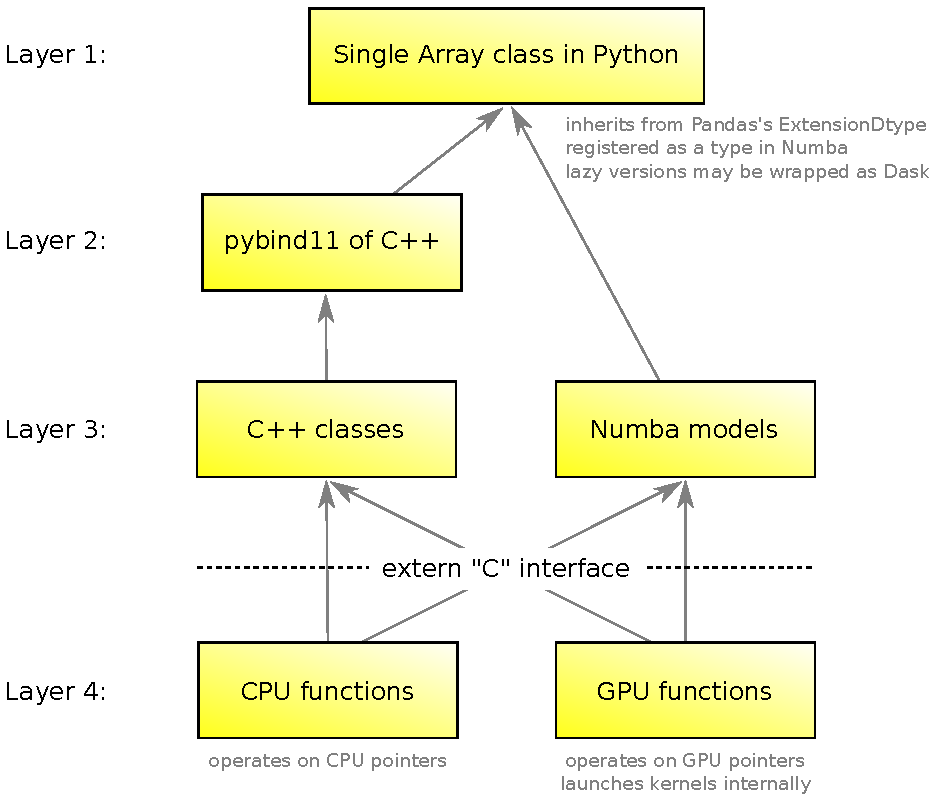
\includegraphics[width=\linewidth]{awkward-1-0-layers.pdf}
\end{columns}
\end{frame}

\begin{frame}[fragile]{Interface changes}
\Large
\vspace{0.25 cm}
Interface changes are not technically coupled to the internal redesign, but I think it's a good time to introduce them.

\normalsize
\vspace{0.5 cm}
\begin{columns}
\column{0.5\linewidth}
\mbox{ } \hfill \textcolor{darkblue}{\Large\underline{Awkward 0.x}} \hfill \mbox{ }

\vspace{0.2 cm}
Structure manipulation and custom physics functions are methods.

\small
\begin{minted}[stripnl=false]{python}

x.cross(y)  # cross-join
x.cross(y)  # 3D cross-product
x.colname   # column data
\end{minted}

\normalsize
\vspace{0.1 cm}
``Layout'' is visible as nested classes.
\vspace{\baselineskip}

\small
\begin{minted}{python}
ChunkedArray(JaggedArray(...))
\end{minted}

\column{0.5\linewidth}
\mbox{ } \hfill \textcolor{darkblue}{\Large\underline{Awkward 1.x}} \hfill \mbox{ }

\vspace{0.2 cm}
Structure manipulation are functions; custom physics functions are methods.

\small
\begin{minted}{python}
import awkward as ak
ak.cross(x, y) # cross-join
x.cross(y)     # 3D cross-product
x.colname      # column data
\end{minted}

\normalsize
\vspace{0.1 cm}
User sees a single \mintinline{python}{Array} class; the layout is hidden inside.

\small
\begin{minted}{python}
Array(...)   # .layout for details
\end{minted}

\end{columns}
\end{frame}

\begin{frame}{Status (after 1 week)}
\vspace{0.5 cm}
\large
\begin{enumerate}\setlength{\itemsep}{0.35 cm}
\item Skeleton for 3 layers: \textcolor{darkorange}{\bf cpu-kernels}, \textcolor{darkorange}{\bf C++}, \textcolor{darkorange}{\bf Python (pybind11)}, \textcolor{darkorange}{\bf Numba}.
\item Compiles/tests on \{Linux, MacOS, Windows\} $\times$ \{Python 2.7, 3.4--3.7\} $\times$ \{Numpy 1.13.1, 1.14.5, latest\}. \textcolor{gray}{(Azure Pipelines are fast!)}
\item Deploys wheels for \{Linux, MacOS, Windows\} $\times$ \{Python 2.7, 3.4--3.7\}.
\item Unified memory management between Python reference count, \mintinline{c++}{std::shared_ptr}, and Numba's ownership model.
\item Basic C++ class and Numba model for \mintinline{python}{ListOffsetArray} with \mintinline{python}{__getitem__(int)} and \mintinline{python}{__getitem__(slice)}.
\end{enumerate}

\vspace{0.5 cm}
\mbox{ } \hfill \textcolor{blue}{\underline{\url{https://github.com/jpivarski/awkward-1.0}}} \hfill \mbox{ }
\end{frame}

\end{document}
